\section{Die Formen des Universums}
Eine der spannendsten Fragen der Kosmologie ist eine ganz simple: Welche Form 
hat unser Universum? Mit Form ist in diesem Kontext die lokale und globale Geometrie
des Universums gemeint. Dabei ist nicht nur die Krümmung des Universums relevant,
sondern auch wie sich die Raumzeit durch Masse und Energie verformt (Dieses Konzept
wurde von Einstein mittels der allgemeinen Relativitätstheorie beschrieben).

Nach der Entdeckung und Messung der kosmischen Mikrowellenhintergrundstrahlung 
ist es uns möglich, diese Frage zu beantworten.
Die Frage nach der Form eines Körpers ist überraschend einfach durch die 
klassische Geometrie zu klären.
Grundsätzlich sind drei mögliche Formen denkbar:
\begin{itemize}
	\item Das Universum könnte positiv gekrümmt sein, wie eine Kugel.
	Zwei parallele Linien auf der Kugeloberfläche kreuzen sich und die 
	Winkelsumme eines Dreiecks ist grösser als $180\degree$ (siehe 
	Längengrade auf der Erdkugel).
	Beim Zurückblicken in der Zeit würde dies zu einem Vergrösserungseffekt 
	führen,
	als würde man durch ein Fernrohr blicken.
	\item Das Universum könnte negativ gekrümmt sein, wie ein Sattel.
	Zwei parallele Linien weichen immer stärker voneinander ab und die 
	Winkelsumme eines Dreiecks ist kleiner als $180\degree$.
	Beim Zurückblicken in der Zeit würde dies zu einem Verkleinerungseffekt 
	führen,
	als würde man auf der falschen Seite durch ein Fernrohr blicken.
	\item Das Universum könnte flach sein, wie ein Blatt Papier.
	Zwei parallele Linien berühren sich nie und die Winkelsumme eines Dreiecks 
	beträgt $180\degree$.
	Beim Zurückblicken, wären die Bilder so, wie wir sie es aufgrund der 
	Berechnungen erwarten %TODO: (wieso? --> erklären).
\end{itemize}
% EINFÜGEN DER BILDER VOM SKRIPT

Diese Effekte würden sich auf die Bilder der kosmischen Mikrowellenhintergrundstrahlung
wie auf Abbildung \ref{fig:universe_shapes} auswirken.
Kurz gesagt, würden sich die Abstände zwischen den Temperatur-Extrema vergrössern, respektive verkürzen.

\begin{figure}
	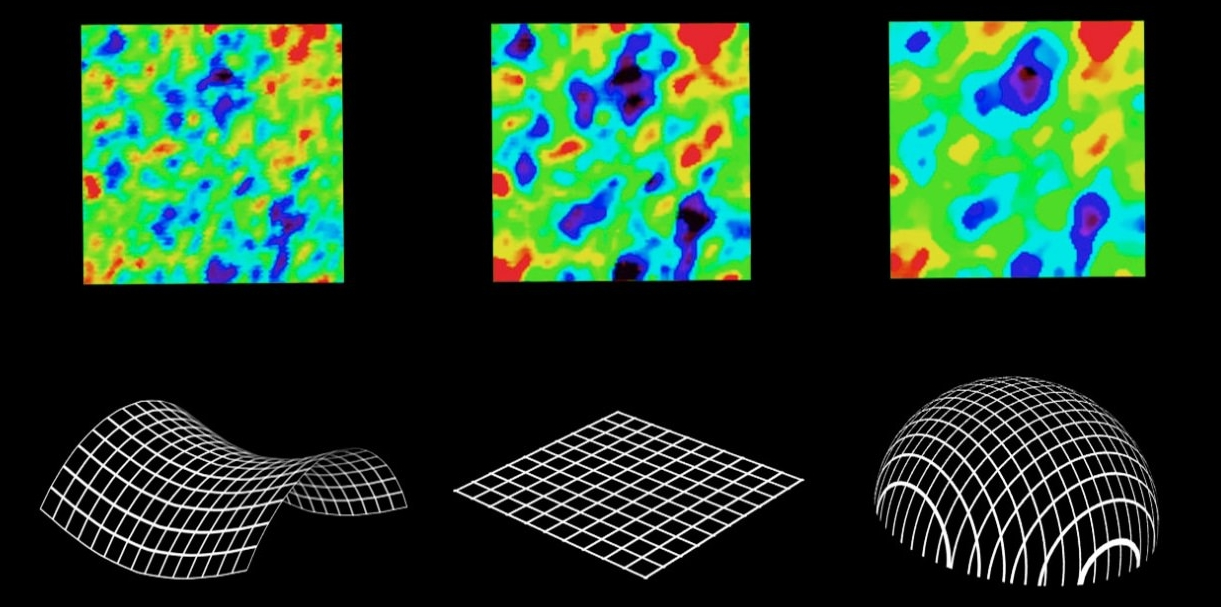
\includegraphics[width=\linewidth]{cmb/images/universe_shapes.jpg}
	\caption{Die drei möglichen Formen des Universums und die daraus 
		resultierenden Bilder des gleichen Ausschnitts der kosmischen
		Mikrowellenhintergrundstrahlung}
	\label{fig:universe_shapes}
\end{figure}

\subsection{Bedeutung der Daten}
Da die Temperaturanisotropien der kosmischen Mikrowellenhintergrundstrahlung auf einer
Kugeloberfläche liegen, sind sie ein sphärisches Problem und man kann sie somit mit 
Kugelflächenfunktionen beschreiben, welche im nächsten Kapitel genauer erläutert werden.
Aus diesen Kugelfunktionen lässt sich herleiten, welche Wellenlängen in welchem Anteil vertreten sind.

Da die Wellenlängen und die Temperatur der kosmischen Hintergrundstrahlung proportional sind, lassen sich die Temperaturanisotropien der Strahlung als Winkelleistungsspektrum darstellen.
Stellt man dieses Spektrum als Funktion des Multipolmoments $l$ dar erhält man 
Abbildung \ref{fig:planck_spectrum}.

\begin{figure}
	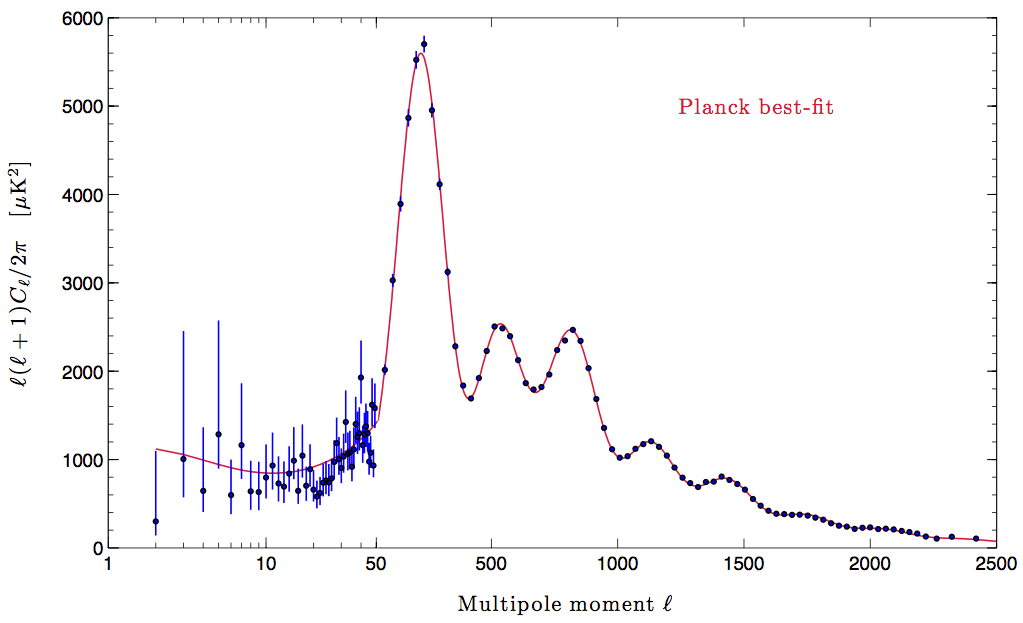
\includegraphics[width=\linewidth]{cmb/images/mission_spectrum.png}
	\caption{Winkelleistungsspektrum der Temperaturanisotropien als Funktion 
	des Multipolmoments $l$.
	Die X-Skala ist logarithmisch bis zu $l = 50$, danach linear. Das Maximum 
	ist bei $l \approx 200$}
	\label{fig:planck_spectrum}
\end{figure}

Die Winkel zwischen den einzelnen Wellen der Strahlung würden bei einem nicht flachen Universum
vergrössert oder verkleinert werden, bzw. von $1\degree$ abweichen. 
%(nachfragen?)
Grosse $l$ entsprechen dabei kleineren Winkeln und kleine $l$ entsprechen 
grösseren Winkeln.
%Formel: Alpha = 180 Grad / l
Die Lage des ersten Peaks findet sich bei rund $1\degree$ und erlaubt es uns 
die Raumkrümmung zu messen.
Bei einer negativen Krümmung des Universums müsste der Peak weiter rechts 
liegen (Alpha $> 1\degree$: Winkelsumme $> 180\degree$),
bei einer positiven Krümmung weiter links (Alpha $< 1\degree$: Winkelsumme $< 
180\degree$).

Daraus folgt: das Universum ist flach.
